\protect\hyperlink{main-nav}{≡} \protect\hyperlink{close-nav}{×}

\hypertarget{section-1.2-operations-on-functions}{%
\section{Section 1.2: Operations on
Functions}\label{section-1.2-operations-on-functions}}

\hypertarget{composition-of-functions}{%
\subsection{Composition of Functions}\label{composition-of-functions}}

Suppose we wanted to calculate how much it costs to heat a house on a
particular day of the year. The cost to heat a house will depend on the
average daily temperature, and the average daily temperature depends on
the particular day of the year. Notice how we have just defined two
relationships: The temperature depends on the day, and the cost depends
on the temperature. Using descriptive variables, we can notate these two
functions.

The first function, \textbackslash{}(C(T)\textbackslash{}), gives the
cost \textbackslash{}(C\textbackslash{}) of heating a house when the
average daily temperature is \textbackslash{}(T\textbackslash{}) degrees
Celsius, and the second, \textbackslash{}(T(d)\textbackslash{}), gives
the average daily temperature of a particular city on day
\textbackslash{}(d\textbackslash{}) of the year. If we wanted to
determine the cost of heating the house on the fifth day of the year, we
could do this by linking our two functions together, an idea called
composition of functions. Using the function
\textbackslash{}(T(d)\textbackslash{}), we could evaluate
\textbackslash{}(T(5)\textbackslash{}) to determine the average daily
temperature on the fifth day of the year. We could then use that
temperature as the input to the \textbackslash{}(C(T)\textbackslash{})
function to find the cost to heat the house on the fifth day of the
year: \textbackslash{}(C(T(5))\textbackslash{}).

\hypertarget{composition-of-functions-1}{%
\paragraph{Composition of Functions}\label{composition-of-functions-1}}

When the output of one function is used as the input of another, we call
the entire operation a composition of functions. We write
\textbackslash{}(f(g(x))\textbackslash{}), and read this as ``f of g of
x'' or ``f composed with g at x''.

An alternate notation for composition uses the composition operator:
\textbackslash{}(\textbackslash{}circ\textbackslash{}).
\textbackslash{}((f\textbackslash{}circ g)(x)\textbackslash{}) is read
``f of g of x'' or ``f composed with g at x'', just like
\textbackslash{}(f(g(x))\textbackslash{}).

\hypertarget{example-1}{%
\paragraph{Example 1}\label{example-1}}

Suppose c(s) gives the number of calories burned doing s sit-ups, and
s(t) gives the number of sit-ups a person can do in t minutes. Interpret
c(s(3)).

When we are asked to interpret, we are being asked to explain the
meaning of the expression in words. The inside expression in the
composition is s(3). Since the input to the s function is time, the 3 is
representing 3 minutes, and s(3) is the number of sit-ups that can be
done in 3 minutes. Taking this output and using it as the input to the
c(s) function will give us the calories that can be burned by the number
of sit-ups that can be done in 3 minutes.

\hypertarget{composition-of-functions-using-tables-and-graphs}{%
\subsubsection{Composition of Functions using Tables and
Graphs}\label{composition-of-functions-using-tables-and-graphs}}

When working with functions given as tables and graphs, we can look up
values for the functions using a provided table or graph. We start
evaluation from the provided input, and first evaluate the inside
function. We can then use the output of the inside function as the input
to the outside function. To remember this, always work from the inside
out.

\hypertarget{example-2}{%
\paragraph{Example 2}\label{example-2}}

Using the graphs below, evaluate
\textbackslash{}(f(g(1))\textbackslash{}) .

\begin{figure}
\centering
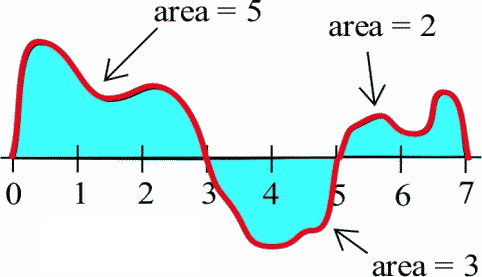
\includegraphics{images/image026.png}
\caption{\textbackslash{}( g(x) \textbackslash{})}
\end{figure}

\begin{figure}
\centering
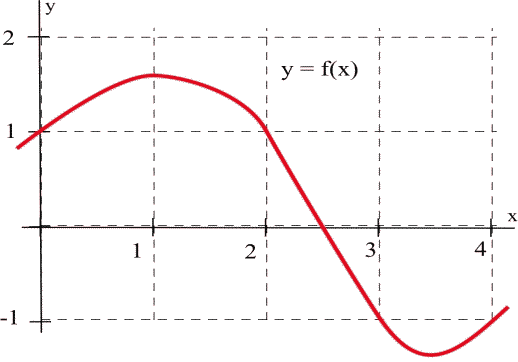
\includegraphics{images/image027.png}
\caption{\textbackslash{}( f(x) \textbackslash{})}
\end{figure}

To evaluate \textbackslash{}(f(g(1))\textbackslash{}), we again start
with the inside evaluation. We evaluate
\textbackslash{}(g(1)\textbackslash{}) using the graph of the
\textbackslash{}(g(x)\textbackslash{}) function, finding the input of 1
on the horizontal axis and finding the output value of the graph at that
input. Here, \textbackslash{}(g(1)=3\textbackslash{}). Using this value
as the input to the \textbackslash{}(f\textbackslash{}) function,
\textbackslash{}(f(g(1))=f(3)\textbackslash{}). We can then evaluate
this by looking to the graph of the
\textbackslash{}(f(x)\textbackslash{}) function, finding the input of 3
on the horizontal axis, and reading the output value of the graph at
this input. Here, \textbackslash{}(f(3)=6\textbackslash{}), so
\textbackslash{}(f(g(1))=6\textbackslash{}).

To view this video please enable JavaScript, and consider upgrading to a
web browser that \href{http://videojs.com/html5-video-support/}{supports
HTML5 video}

\hypertarget{compositions-using-formulas}{%
\subsubsection{Compositions using
Formulas}\label{compositions-using-formulas}}

When evaluating a composition of functions where we have either created
or been given formulas, the concept of working from the inside out
remains the same. First we evaluate the inside function using the input
value provided, then use the resulting output as the input to the
outside function.

\hypertarget{example-3}{%
\paragraph{Example 3}\label{example-3}}

Given \textbackslash{}(f(t)=t\^{}2-t\textbackslash{}) and
\textbackslash{}(h(x)=3x+2\textbackslash{}), evaluate
\textbackslash{}(f(h(1))\textbackslash{}).

Since the inside evaluation is \textbackslash{}(h(1)\textbackslash{}) we
start by evaluating the \textbackslash{}(h(x)\textbackslash{}) function
at 1: \textbackslash{}{[}h(1)=3(1)+2=5\textbackslash{}{]}

Then \textbackslash{}(f(h(1))=f(5)\textbackslash{}) , so we evaluate the
\textbackslash{}(f(t)\textbackslash{}) function at an input of 5:
\textbackslash{}{[}f(h(1))=f(5)=5\^{}2-5=20\textbackslash{}{]}

We are not limited, however, to using a numerical value as the input to
the function. We can put anything into the function: a value, a
different variable, or even an algebraic expression, provided we use the
input expression everywhere we see the input variable.

\hypertarget{example-4}{%
\paragraph{Example 4}\label{example-4}}

Let \textbackslash{}(f(x)=x\^{}2\textbackslash{}) and
\textbackslash{}(g(x)=\textbackslash{}dfrac\{1\}\{x\}-2x\textbackslash{}).
Find \textbackslash{}(f(g(x))\textbackslash{}) and
\textbackslash{}(g(f(x))\textbackslash{}).

To find \textbackslash{}(f(g(x))\textbackslash{}), we start by
evaluating the inside, writing out the formula for
\textbackslash{}(g(x)\textbackslash{}):\textbackslash{}{[}g(x)=\textbackslash{}dfrac\{1\}\{x\}-2x\textbackslash{}{]}

We then use the expression
\textbackslash{}(\textbackslash{}left(\textbackslash{}dfrac\{1\}\{x\}-2x\textbackslash{}right)\textbackslash{})
as the input for the function \textbackslash{}(f\textbackslash{}):
\textbackslash{}{[}f(g(x))=f\textbackslash{}left(\textbackslash{}dfrac\{1\}\{x\}-2x\textbackslash{}right)\textbackslash{}{]}

We then evaluate the function \textbackslash{}(f(x)\textbackslash{})
using the formula for \textbackslash{}(g(x)\textbackslash{}) as the
input. Since \textbackslash{}(f(x)=x\^{}2\textbackslash{}) then
\textbackslash{}{[}f\textbackslash{}left(\textbackslash{}dfrac\{1\}\{x\}-2x\textbackslash{}right)=\textbackslash{}left(\textbackslash{}dfrac\{1\}\{x\}-2x\textbackslash{}right)\^{}2\textbackslash{}{]}

This gives us the formula for the composition:
\textbackslash{}{[}f(g(x))=\textbackslash{}left(\textbackslash{}dfrac\{1\}\{x\}-2x\textbackslash{}right)\^{}2\textbackslash{}{]}

Likewise, to find \textbackslash{}(g(f(x))\textbackslash{}), we evaluate
the inside, writing out the formula for
\textbackslash{}(f(x)\textbackslash{}):
\textbackslash{}(g(f(x))=g(x\^{}2)\textbackslash{}). Now we evaluate the
function \textbackslash{}(g(x)\textbackslash{}) using
\textbackslash{}(x\^{}2\textbackslash{}) as the input:
\textbackslash{}{[}g(f(x))=\textbackslash{}dfrac\{1\}\{x\^{}2\}-2x\^{}2\textbackslash{}{]}

To view this video please enable JavaScript, and consider upgrading to a
web browser that \href{http://videojs.com/html5-video-support/}{supports
HTML5 video}

\hypertarget{example-5}{%
\paragraph{Example 5}\label{example-5}}

A city manager determines that the tax revenue,
\textbackslash{}(R\textbackslash{}), in millions of dollars collected on
a population of \textbackslash{}(p\textbackslash{}) thousand people is
given by the formula
\textbackslash{}(R(p)=0.03p+\textbackslash{}sqrt\{p\}\textbackslash{}),
and that the city's population, in thousands, is predicted to follow the
formula \textbackslash{}(p(t)=60+2t+0.3t\^{}2\textbackslash{}), where
\textbackslash{}(t\textbackslash{}) is measured in years after 2010.
Find a formula for the tax revenue as a function of the year.

Since we want tax revenue as a function of the year, we want year to be
our initial input, and revenue to be our final output. To find revenue,
we will first have to predict the city population, and then use that
result as the input to the tax function. So we need to find
\textbackslash{}(R(p(t)).\textbackslash{}) Evaluating this,
\textbackslash{}{[}\textbackslash{}begin\{align*\} R(p(t)) =\&
R(60+2t+0.3t\^{}2)\textbackslash{}\textbackslash{} =\&
0.03(60+2t+0.3t\^{}2)+\textbackslash{}sqrt\{60+2t+0.3t\^{}2\}
\textbackslash{}end\{align*\}\textbackslash{}{]}

This composition gives us a single formula which can be used to predict
the tax revenue during a given year, without needing to find the
intermediary population value. For example, to predict the tax revenue
in 2017, when t = 7 (because t is measured in years after 2010),
\textbackslash{}{[}\textbackslash{}begin\{align*\} R(p(7)) =\&
0.03\textbackslash{}left(60+2(7)+0.3\textbackslash{}left(7\^{}2\textbackslash{}right)\textbackslash{}right)+\textbackslash{}sqrt\{60+2(7)+0.3\textbackslash{}left(7\^{}2\textbackslash{}right)\}\textbackslash{}\textbackslash{}
\textbackslash{}approx \& 12.079\textbackslash{}text\{ million dollars\}
\textbackslash{}end\{align*\}\textbackslash{}{]}

Later in this course, it will be desirable to decompose a function -- to
write it as a composition of two simpler functions.

\hypertarget{example-6}{%
\paragraph{Example 6}\label{example-6}}

Write
\textbackslash{}(f(x)=3+\textbackslash{}sqrt\{5-x\^{}2\}\textbackslash{})
as the composition of two functions.

We are looking for two functions, \textbackslash{}(g\textbackslash{})
and \textbackslash{}(h\textbackslash{}), so
\textbackslash{}(f(x)=g(h(x))\textbackslash{}). To do this, we look for
a function inside a function in the formula for
\textbackslash{}(f(x)\textbackslash{}). As one possibility, we might
notice that \textbackslash{}(5-x\^{}2\textbackslash{}) is the inside of
the square root. We could then decompose the function as:
\textbackslash{}{[}h(x)=5-x\^{}2, \textbackslash{}quad
g(x)=3+\textbackslash{}sqrt\{x\}\textbackslash{}{]}

We can check our answer by recomposing the functions:
\textbackslash{}{[}g(h(x))=g(5-x\^{}2)=3+\textbackslash{}sqrt\{5-x\^{}2\}\textbackslash{}{]}

Note that this is not the only solution to the problem. Another
non-trivial decomposition would be \textbackslash{}{[}h(x)=x\^{}2,
\textbackslash{}quad
g(x)=3+\textbackslash{}sqrt\{5-x\}.\textbackslash{}{]}

To view this video please enable JavaScript, and consider upgrading to a
web browser that \href{http://videojs.com/html5-video-support/}{supports
HTML5 video}

\hypertarget{transformations-of-functions}{%
\subsection{Transformations of
Functions}\label{transformations-of-functions}}

Transformations allow us to construct new equations from our basic
toolkit functions. The most basic transformations are shifting the graph
vertically or horizontally.

\hypertarget{vertical-shift}{%
\paragraph{Vertical Shift}\label{vertical-shift}}

Given a function \textbackslash{}(f(x)\textbackslash{}), if we define a
new function \textbackslash{}(g(x)\textbackslash{}) as
\textbackslash{}(g(x)=f(x)+k\textbackslash{}), where
\textbackslash{}(k\textbackslash{}) is a constant, then
\textbackslash{}(g(x)\textbackslash{}) is a \textbf{vertical shift} of
the function \textbackslash{}(f(x)\textbackslash{}), where all the
output values have been increased by
\textbackslash{}(k\textbackslash{}).

If \textbackslash{}(k\textbackslash{}) is positive, then the graph will
shift up. If \textbackslash{}(k\textbackslash{}) is negative, then the
graph will shift down.

To view this video please enable JavaScript, and consider upgrading to a
web browser that \href{http://videojs.com/html5-video-support/}{supports
HTML5 video}

\hypertarget{horizontal-shift}{%
\paragraph{Horizontal Shift}\label{horizontal-shift}}

Given a function \textbackslash{}(f(x)\textbackslash{}), if we define a
new function \textbackslash{}(g(x)\textbackslash{}) as
\textbackslash{}(g(x)=f(x+k)\textbackslash{}), where
\textbackslash{}(k\textbackslash{}) is a constant, then
\textbackslash{}(g(x)\textbackslash{}) is a \textbf{horizontal shift} of
the function \textbackslash{}(f(x)\textbackslash{}), where all the
output values have been increased by
\textbackslash{}(k\textbackslash{}).

If \textbackslash{}(k\textbackslash{}) is positive, then the graph will
shift left. If \textbackslash{}(k\textbackslash{}) is negative, then the
graph will shift right.

To view this video please enable JavaScript, and consider upgrading to a
web browser that \href{http://videojs.com/html5-video-support/}{supports
HTML5 video}

\hypertarget{example-7}{%
\paragraph{Example 7}\label{example-7}}

Given \textbackslash{}(f(x)=\textbar{}x\textbar{}\textbackslash{}),
sketch a graph of
\textbackslash{}(h(x)=f(x+1)-3=\textbar{}x+1\textbar{}-3\textbackslash{}).

The function \textbackslash{}(\textbackslash{}) is our toolkit absolute
value function. We know that this graph has a V shape, with the point at
the origin. The graph of \textbackslash{}(h\textbackslash{}) has
transformed \textbackslash{}(f\textbackslash{}) in two ways:
\textbackslash{}(f(x+1)\textbackslash{}) is a change on the inside of
the function, giving a horizontal shift left by 1, then the subtraction
by 3 in \textbackslash{}(f(x+1)-3\textbackslash{}) is a change to the
outside of the function, giving a vertical shift down by 3. Transforming
the graph gives:

\begin{figure}
\centering
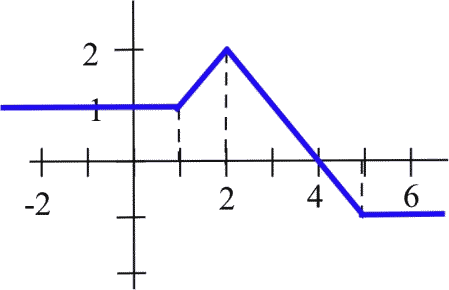
\includegraphics{images/image028.png}
\caption{}
\end{figure}

\hypertarget{example-8}{%
\paragraph{Example 8}\label{example-8}}

Write a formula for the graph shown, a transformation of the toolkit
square root function.

\begin{figure}
\centering
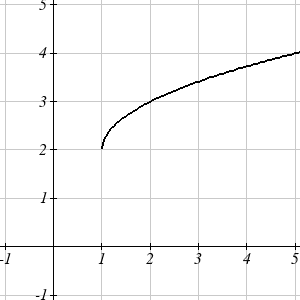
\includegraphics{images/image029.png}
\caption{}
\end{figure}

The graph of the toolkit function starts at the origin, so this graph
has been shifted 1 to the right, and up 2. In function notation, we
could write that as \textbackslash{}(h(x)=f(x-1)+2\textbackslash{}).
Using the formula for the square root function we can write
\textbackslash{}(h(x)=\textbackslash{}sqrt\{x-1\}+2\textbackslash{}).

Note that this transformation has changed the domain and range of the
function. This new graph has domain
\textbackslash{}({[}1,\textbackslash{}infty)\textbackslash{}) and range
\textbackslash{}({[}2,\textbackslash{}infty)\textbackslash{}).

Another transformation that can be applied to a function is a reflection
over the horizontal or vertical axis.

\hypertarget{reflections}{%
\paragraph{Reflections}\label{reflections}}

Given a function \textbackslash{}(f(x)\textbackslash{}), if we define a
new function \textbackslash{}(g(x)\textbackslash{}) as
\textbackslash{}(-f(x)\textbackslash{}), then
\textbackslash{}(g(x)\textbackslash{}) is a \textbf{vertical reflection}
of the function \textbackslash{}(f(x)\textbackslash{}), sometimes called
a reflection about the x-axis

If we define a new function \textbackslash{}(g(x)\textbackslash{}) as
\textbackslash{}(f(-x)\textbackslash{}), then
\textbackslash{}(g(x)\textbackslash{}) is a \textbf{horizontal
reflection} of the function \textbackslash{}(f(x)\textbackslash{}),
sometimes called a reflection about the
\textbackslash{}(y\textbackslash{})-axis.

\hypertarget{example-9}{%
\paragraph{Example 9}\label{example-9}}

A common model for learning has an equation similar to
\textbackslash{}(k(t)=-2\^{}t+1\textbackslash{}) , where
\textbackslash{}(k\textbackslash{}) is the percentage of mastery that
can be achieved after \textbackslash{}(t\textbackslash{}) practice
sessions. This is a transformation of the function
\textbackslash{}(f(t)=2\^{}t\textbackslash{}) shown here. Sketch a graph
of \textbackslash{}(k(t)\textbackslash{}).

\begin{figure}
\centering
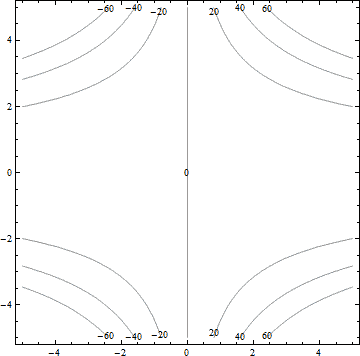
\includegraphics{images/image030.png}
\caption{\textbackslash{}(f(t)=2\^{}t\textbackslash{})}
\end{figure}

This equation combines three transformations into one equation.

\begin{longtable}[]{@{}lll@{}}
\toprule
\endhead
A horizontal reflection: &
\textbackslash{}(f(-t)=2\^{}\{-t\}\textbackslash{}) & combined
with\tabularnewline
a vertical reflection: &
\textbackslash{}(-f(-t)=-2\^{}\{-t\}\textbackslash{}) & combined
with\tabularnewline
a vertical shift up 1: &
\textbackslash{}(-f(-t)+1=-2\^{}\{-t\}+1\textbackslash{}).
&\tabularnewline
\bottomrule
\end{longtable}

We can sketch a graph by applying these transformations one at a time to
the original function:

\begin{figure}
\centering
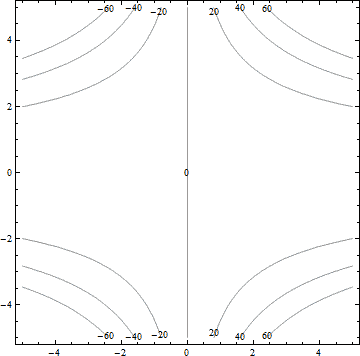
\includegraphics{images/image030.png}
\caption{The original graph}
\end{figure}

\begin{figure}
\centering
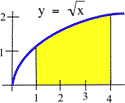
\includegraphics{images/image031.png}
\caption{Horizontally reflected}
\end{figure}

\begin{figure}
\centering
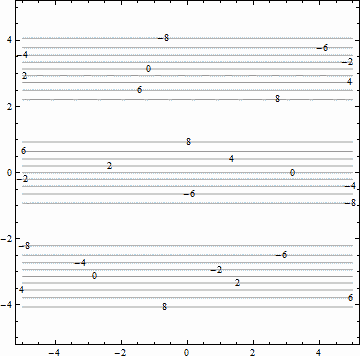
\includegraphics{images/image032.png}
\caption{Then vertically reflected}
\end{figure}

Then, after shifting up 1, we get the final graph:
\textbackslash{}{[}k(t)=-f(-t)+1=-2\^{}\{-t\}+1\textbackslash{}{]}

\begin{figure}
\centering
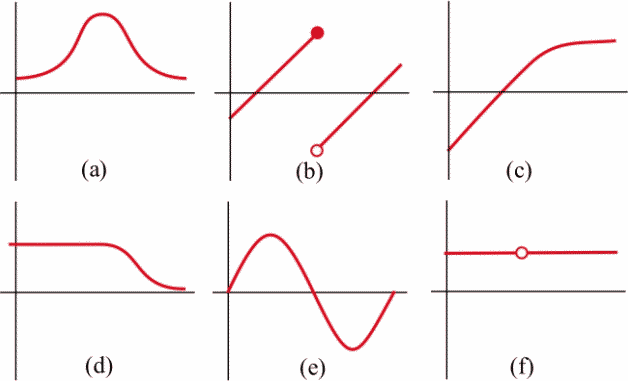
\includegraphics{images/image033.png}
\caption{Final graph}
\end{figure}

Note: As a model for learning, this function would be limited to a
domain of \textbackslash{}(t\textbackslash{}geq 0\textbackslash{}), with
corresponding range \textbackslash{}({[}0,1)\textbackslash{}).

With shifts, we saw the effect of adding or subtracting to the inputs or
outputs of a function. We now explore the effects of multiplying the
outputs.

\hypertarget{vertical-stretchcompression}{%
\paragraph{Vertical
Stretch/Compression}\label{vertical-stretchcompression}}

Given a function \textbackslash{}(f(x)\textbackslash{}), if we define a
new function \textbackslash{}(g(x)\textbackslash{}) as
\textbackslash{}(g(x)=k\textbackslash{}cdot f(x)\textbackslash{}), where
k is a constant, then \textbackslash{}(g(x)\textbackslash{}) is a
\textbf{vertical stretch or compression} of the function
\textbackslash{}(f(x)\textbackslash{}).

\begin{itemize}
\tightlist
\item
  If \textbackslash{}(k \textbackslash{}gt 1\textbackslash{}), then the
  graph will be stretched
\item
  If \textbackslash{}(0\textbackslash{}lt k \textbackslash{}lt
  1\textbackslash{}), then the graph will be compressed
\item
  If \textbackslash{}(k \textbackslash{}lt 0\textbackslash{}), then
  there will be combination of a vertical stretch or compression with a
  vertical reflection
\end{itemize}

To view this video please enable JavaScript, and consider upgrading to a
web browser that \href{http://videojs.com/html5-video-support/}{supports
HTML5 video}

\hypertarget{example-10}{%
\paragraph{Example 10}\label{example-10}}

The graph below is a transformation of the toolkit function
\textbackslash{}(f(x)=x\^{}3\textbackslash{}). Relate this new function
\textbackslash{}(g(x)\textbackslash{}) to
\textbackslash{}(f(x)\textbackslash{}), then find a formula for
\textbackslash{}(g(x)\textbackslash{}).

\begin{figure}
\centering
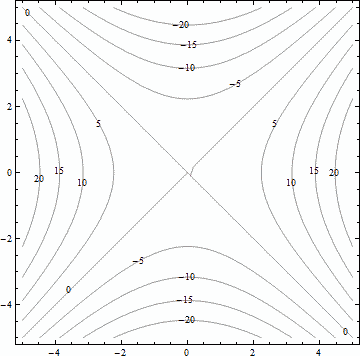
\includegraphics{images/image034.png}
\caption{}
\end{figure}

When trying to determine a vertical stretch or shift, it is helpful to
look for a point on the graph that is relatively clear. In this graph,
it appears that \textbackslash{}(g(2)=2\textbackslash{}). With the basic
cubic function at the same input,
\textbackslash{}(f(2)=2\^{}3=8\textbackslash{}). Based on that, it
appears that the outputs of \textbackslash{}(g\textbackslash{}) are
\textbackslash{}(\textbackslash{}frac\{1\}\{4\}\textbackslash{}) the
outputs of the function \textbackslash{}(f\textbackslash{}), since
\textbackslash{}(g(2)=\textbackslash{}frac\{1\}\{4\}f(x)\textbackslash{}).
From this we can fairly safely conclude that
\textbackslash{}{[}g(x)=\textbackslash{}frac\{1\}\{4\}f(x).\textbackslash{}{]}

We can write a formula for \textbackslash{}(g\textbackslash{}) by using
the definition of the function \textbackslash{}(f\textbackslash{}):
\textbackslash{}{[}g(x)=\textbackslash{}frac\{1\}\{4\}f(x)=\textbackslash{}frac\{1\}\{4\}x\^{}3.\textbackslash{}{]}

\hypertarget{combining-transformations}{%
\subsubsection{Combining
Transformations}\label{combining-transformations}}

When combining vertical transformations, it is very important to
consider the order of the transformations. For example, vertically
shifting by 3 and then vertically stretching by 2 does not create the
same graph as vertically stretching by 2 and then vertically shifting by
3. The order follows nicely from order of operations.

\hypertarget{combining-vertical-transformations}{%
\paragraph{Combining Vertical
Transformations}\label{combining-vertical-transformations}}

When combining vertical transformations written in the form
\textbackslash{}(a\textbackslash{}cdot f(x)+k\textbackslash{}), first
vertically stretch by \textbackslash{}(a\textbackslash{}), then
vertically shift by \textbackslash{}(k\textbackslash{}).

\hypertarget{example-11}{%
\paragraph{Example 11}\label{example-11}}

Write an equation for the transformed graph of the quadratic function
shown.

\begin{figure}
\centering
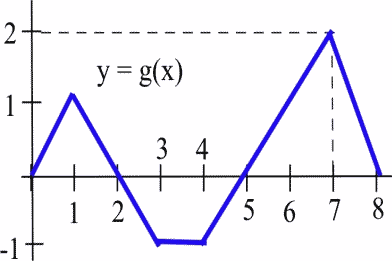
\includegraphics{images/image035.png}
\caption{}
\end{figure}

Since this is a quadratic function, first consider what the basic
quadratic tool kit function looks like and how this has changed.
Observing the graph, we notice several transformations: The original
tool kit function has been flipped over the x axis, some kind of stretch
or compression has occurred, and we can see a shift to the right 3 units
and a shift up 1 unit. In total there are four operations:

\begin{enumerate}
\tightlist
\item
  Vertical Reflection, requiring a negative sign outside the function.
\item
  Vertical Stretch
\item
  Horizontal Shift Right 3 units, which tells us to put x-3 on the
  inside of the function.
\item
  Vertical Shift up 1 unit, telling us to add 1 on the outside of the
  function.
\end{enumerate}

By observation, the basic tool kit function has a vertex at (0, 0) and
symmetrical points at (1, 1) and (-1, 1). These points are 1 unit up and
1 unit over from the vertex. The new points on the transformed graph are
1 unit away horizontally but 2 units away vertically. They have been
stretched vertically by 2.

Not everyone can see this by simply looking at the graph. If you can,
great, but if not we can solve for it. First, we will write the equation
for this graph, with an unknown vertical stretch:

\begin{longtable}[]{@{}ll@{}}
\toprule
\endhead
\textbackslash{}(f(x)=x\^{}2\textbackslash{}) & The original
function\tabularnewline
\textbackslash{}(-f(x)=-x\^{}2\textbackslash{}) & Vertically
reflected\tabularnewline
\textbackslash{}(-a\textbackslash{}cdot f(x)=-a x\^{}2\textbackslash{})
& Vertically stretched\tabularnewline
\textbackslash{}(-a\textbackslash{}cdot
f(x-3)=-a(x-3)\^{}2\textbackslash{}) & Shifted right 3\tabularnewline
\textbackslash{}(-a\textbackslash{}cdot
f(x-3)+1=-a(x-3)\^{}2+1\textbackslash{}) & Shifted up 1\tabularnewline
\bottomrule
\end{longtable}

We now know our graph is going to have an equation of the form
\textbackslash{}(g(x)=-a(x-3)\^{}2+1\textbackslash{}). To find the
vertical stretch, we can identify any point on the graph (other than the
highest point), such as the point (2,-1), which tells us
\textbackslash{}(g(2)=-1\textbackslash{}). Using our general formula,
and substituting 2 for \textbackslash{}(x\textbackslash{}), and -1 for
\textbackslash{}(g(x)\textbackslash{}).

This tells us that to produce the graph we need a vertical stretch by
two.

Thus the function that produces this graph is
\textbackslash{}{[}g(x)=-2(x-3)\^{}2+1.\textbackslash{}{]}

To view this video please enable JavaScript, and consider upgrading to a
web browser that \href{http://videojs.com/html5-video-support/}{supports
HTML5 video}

\hypertarget{example-12}{%
\paragraph{Example 12}\label{example-12}}

On what interval(s) is the function
\textbackslash{}(g(x)=\textbackslash{}dfrac\{-2\}\{(x-1)\^{}2\}+3\textbackslash{})
increasing and decreasing?

This is a transformation of the toolkit reciprocal squared function,
\textbackslash{}(f(x)=\textbackslash{}dfrac\{1\}\{x\^{}2\}\textbackslash{})

\begin{longtable}[]{@{}ll@{}}
\toprule
\endhead
\textbackslash{}(-2f(x)=\textbackslash{}dfrac\{-2\}\{x\^{}2\}\textbackslash{})
& A vertical flip and vertical stretch by 2\tabularnewline
\textbackslash{}(-2f(x-1)=\textbackslash{}dfrac\{-2\}\{(x-1)\^{}2\}\textbackslash{})
& A shift right by 1\tabularnewline
\textbackslash{}(-2f(x-1)+3=\textbackslash{}dfrac\{-2\}\{(x-1)\^{}2\}+3\textbackslash{})
& A shift up by 3\tabularnewline
\bottomrule
\end{longtable}

The basic reciprocal squared function is increasing on
\textbackslash{}((-\textbackslash{}infty,0)\textbackslash{}) and
decreasing on
\textbackslash{}((0,\textbackslash{}infty)\textbackslash{}). Because of
the vertical flip, the \textbackslash{}(g(x)\textbackslash{}) function
will be decreasing on the left and increasing on the right. The
horizontal shift right by 1 will also shift these intervals to the right
one. From this, we can determine \textbackslash{}(g(x)\textbackslash{})
will be increasing on
\textbackslash{}((1,\textbackslash{}infty)\textbackslash{}) and
decreasing on
\textbackslash{}((-\textbackslash{}infty,1)\textbackslash{}). We also
could graph the transformation to help us determine these intervals.

\begin{figure}
\centering
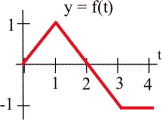
\includegraphics{images/image036.png}
\caption{Graph of the transformed function.}
\end{figure}

\begin{longtable}[]{@{}ll@{}}
\toprule
\endhead
\href{section1-1.php}{← Previous Section} & \href{section1-3.php}{Next
Section →}\tabularnewline
\bottomrule
\end{longtable}
